\documentclass{article}
% translate with >> pdflatex -shell-escape <file>

% This file is an extract of the PGFPLOTS manual, copyright by Christian Feuersaenger.
% 
% Feel free to use it as long as you cite the pgfplots manual properly.
%
% See
%   http://pgfplots.sourceforge.net/pgfplots.pdf
% for the complete manual.
%
% Any required input files (for <plot table> or <plot file> or the table package) can be downloaded
% at
% http://www.ctan.org/tex-archive/graphics/pgf/contrib/pgfplots/doc/latex/
% and
% http://www.ctan.org/tex-archive/graphics/pgf/contrib/pgfplots/doc/latex/plotdata/

\usepackage{pgfplots}
\pgfplotsset{compat=newest}

\pagestyle{empty}

\usepgfplotslibrary{ternary}

\begin{document}
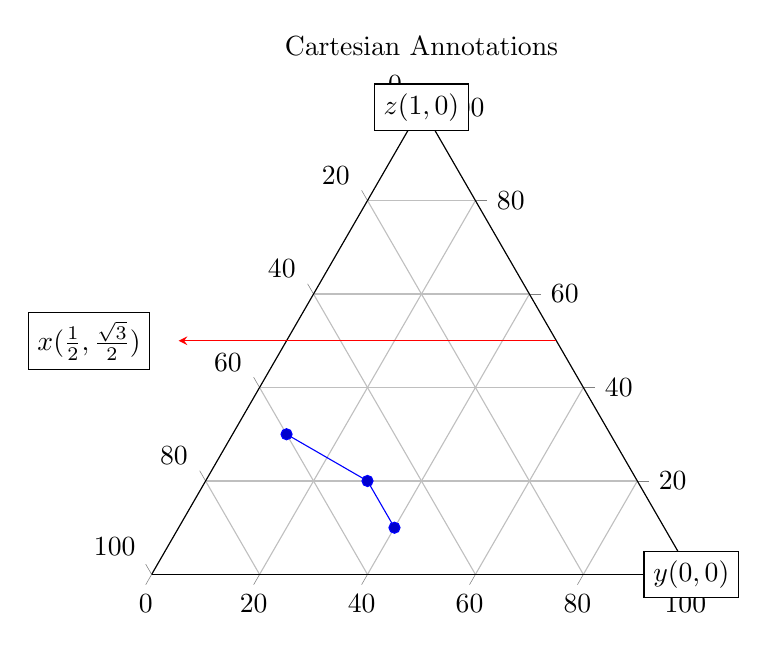
\begin{tikzpicture}
	\begin{ternaryaxis}[
		title=Cartesian Annotations,
		clip=false]

	\addplot3 coordinates {
		(0.1,0.5,0.4)
		(0.2,0.5,0.3)
		(0.3,0.6,0.1)
	};

	\node[fill=white,draw] at (0,0) {$y (0,0)$};
	\node[fill=white,draw] at (1,0) {$z (1,0)$};
	\node[fill=white,draw] at (0.5,{sqrt(3)/2}) 
		{$x (\frac12,\frac{\sqrt3}{2})$};
	
	\draw[red,-stealth] (0.5,0) -- (0.5,0.7);
	\end{ternaryaxis}
\end{tikzpicture}
\end{document}
